\documentclass[9pt]{article} \usepackage{amsmath, amsthm, amssymb}
\usepackage{array,mathtools} \usepackage[textwidth=8in,textheight=9in]{geometry} %
\newcommand\showdiv[1]{\overline{\smash{\hstretch{.5}{)}\mkern-3.2mu\hstretch{.5}{)}}#1}} %
\newcommand\ph[1]{\textcolor{white}{#1}} %
\newcommand*{\carry}[1][1]{\overset{#1}} % \newcolumntype{B}[1]{r*{#1}{@{\,}r}}
\usepackage{tikz}
\def\checkmark{\tikz\fill[scale=0.4](0,.35) -- (.25,0) -- (1,.7) -- (.25,.15) -- cycle;}
\usepackage{amsmath}
\usepackage{listings} \usepackage{courier} \setlength{\oddsidemargin}{-1cm}
\setlength{\evensidemargin}{0cm} \setlength{\textwidth}{500pt}
\newenvironment{Figure}
  {\par\medskip\noindent\minipage{\linewidth}}
  {\endminipage\par\medskip}
\usepackage{multicol,caption}
\usepackage{color} \usepackage{wrapfig} \usepackage{url}
\usepackage[parfill]{parskip}
\usepackage{listings} \usepackage{color}
\usepackage[font=small,labelfont=bf]{caption}

\definecolor{mygreen}{rgb}{0,0.6,0} \definecolor{mygray}{rgb}{0.5,0.5,0.5}
\definecolor{mymauve}{rgb}{0.58,0,0.82}

\usepackage{courier}

\lstset{basicstyle=\footnotesize\ttfamily,breaklines=true}
\lstset{framextopmargin=50pt,frame=bottomline}

\title{{Background \& Progress Report}\\{\large Semi-Supervised Facial Action Unit Recogniton with Deep Neural Networks}}
\author{Luka Milic: lm1015}

\begin{document}
\maketitle

\begin{abstract}
    Deep neural networks typically require large amounts of labelled data to make useful
    predictions, however in most domains this data is rare and mainly unlabelled.
    This project aims to incorporate that unlabelled data into a deep learning algorithm.
    A network with an autoencoder and classifier is proposed to be able to simultaneously
    learn from labelled and unlabelled data in a semi-supervised way. Detecting
    facial actions units is the chosen domain to benchmark this approach, with
    the DISFA dataset being used for preliminary experiments.
\end{abstract}
%
%
%
\tableofcontents
\section{Background}
\subsection{Introduction}
The human face is most likely one of the most researched objects in image analysis
and computer vision \cite{S.ZafeiriouA.PapaioannouI.KotsiaM.A.Nicolaou}.
It has wide ranging applications from Human
Computer Interaction (expression recognition) to law enforcement (face recognition).
Its study also necessitates the development of a wide range of machine
learning algorithms, in areas such as bayesian inference and deep learning.

There exist many datasets containing images and videos of faces and it is a general
observation that unlabelled datasets are far more abundant than labelled ones.
In particular in the areas of expression recognition where painstaking work
must be carried out to obtain the ground truth expressions for an image or set of
frames in a video.

\begin{figure}
 \centering
 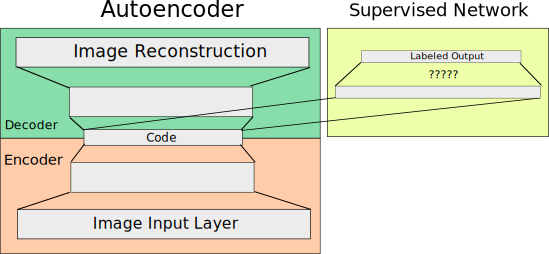
\includegraphics[width=0.5\textwidth]{illustrations/network_01.pdf}
 \captionof{figure}{General structure of the proposed network. Each rectangle
 represents many layers of neurons and the thin lines represent connections between layers.}
\end{figure}

Facial Action Unit detection FAU \cite{Corneanu2016} is chosen in this work due
to it's popularity and available benchmarks.
The Facial Action Coding System (FACS) developed by Ekman and Friesen,
provides a systematic way to study any kind of facial expression,
by representing them as a combination of individual facial muscle actions
known as Action Units (AU). Automating the process of detecting AUs is difficult
because they have non-linear interactions and often occur in very low intensities.

Deep learning is emerging as a powerful tool in modelling a wide range of patterns
in data, it has been applied to the problem of FAU a number of times and achieved
good classification rates. One complication which arises when using Deep Neural
Networks DNNs to classify AUs is that many frames are unlabelled (have neutral expressions)
and hence the standard supervised DNN do not make good use of this information.
This project aims to investigate how an autoencoder could be combined with the
already established deep learning methods related to FAU in order to improve the performance
of these techniques and better leverage unlabelled data. This unlabelled data may
come from within the standard AU datasets or from larger databases of faces.
The DISFA dataset is chosen for initial experiments.

\subsection{Related Work}

\subsubsection{Databases and Benchmarks for FAU estimation}
Relevant for this work is a awareness of datasets which exist and may be useful
for experiments. Here is a list of some which should be used in order to allow
this project to be comparable to work in the literature:

\begin{itemize}
    \item CK+ \cite{Lucey2010} containing 123 subjects recorded with faces in strictly front positions.
    \item The DISFA database \cite{disfa}, which contains only 27 people whose spontaneous
          facial expressions were captured in controlled recording conditions.
    \item FERA 2015 BP4D-Spontaneous Dataset \cite{Valstar}:
          It consists of 41 subjects and 34 AUs, and the subjects were young adults who
          spontaneously generated emotional responses to stimulus tasks.
\end{itemize}

This is just a small selection, however is it representative of the types of
datasets available. Each frame of the videos has a label which describes which AUs are
present and their intensity. Hence two distinct problems can be tackled here, intensity
estimation and classification, this work follows the classification route however
intensity estimation should also be possible with a few minor modifications.

A key challenge with these datasets is that they often have very unbalanced and
sparse labels as shown in figure \ref{disfastats}. This calls for methods
to balance training samples with respect to this imbalance and is the
motivation for using some unsupervised learning techniques, in order to extract information
from the unlabelled data.

A further two datasets are the TFD and SEMAINE, these do not contain AUs but often crop up in the
literature:
\begin{itemize}
     \item TFD \cite{tfd} Toronto Face Dataset
     \item The SEMAINE \cite{semaine} corpus which contains recordings
           of people interacting with a Sensitive Artificial Listener (SAL) in controlled conditions.
\end{itemize}

\subsubsection{The DISFA dataset} \label{disfa_list}
Of particular interest to the project is the DISFA dataset, it has 27 subjects with 12 AUs.
Each frame in each subject video has a label which says how much of each AU is present on
a scale of 0-5, the distribution of intensities is shown in table \ref{compau}.

A challenge of the DISFA dataset is that it has many frames which are unlabelled, this is demonstrated
per subject in figure \ref{disfastats}. Many of the subjects have over 40\% of their frames unlabelled
, one outlier has over 75\% unlabelled.

\begin{table}[h!]
\centering

\begin{tabular}{lllllll}
\hline
Intensity & 0      & 1     & 2     & 3     & 4    & 5    \\ \hline
AU1       & 112286 & 2272  & 1749  & 2809  & 1393 & 555  \\
AU2       & 99165  & 1720  & 934   & 3505  & 836  & 369  \\
AU4       & 106160 & 4661  & 7636  & 6586  & 4328 & 1383 \\
AU5       & 99015  & 1579  & 719   & 293   & 104  & 34   \\
AU6       & 106425 & 9157  & 5986  & 3599  & 601  & 141  \\
AU9       & 99458  & 1659  & 2035  & 3045  & 316  & 77   \\
AU12      & 99987  & 13943 & 6869  & 7233  & 2550 & 172  \\
AU15      & 108358 & 5180  & 1618  & 1017  & 47   & 0    \\
AU17      & 117824 & 6342  & 4184  & 2281  & 112  & 11   \\
AU20      & 121377 & 1591  & 1608  & 1305  & 28   & 0    \\
AU25      & 84721  & 9805  & 13935 & 15674 & 5580 & 1039 \\
AU26      & 105778 & 13443 & 7473  & 3529  & 314  & 217  \\ \hline
\end{tabular}
\caption{A comparison of the number of occurrences of each intensity for each AU in the DISFA dataset} \label{compau}
\end{table}


\begin{figure}[h!]
  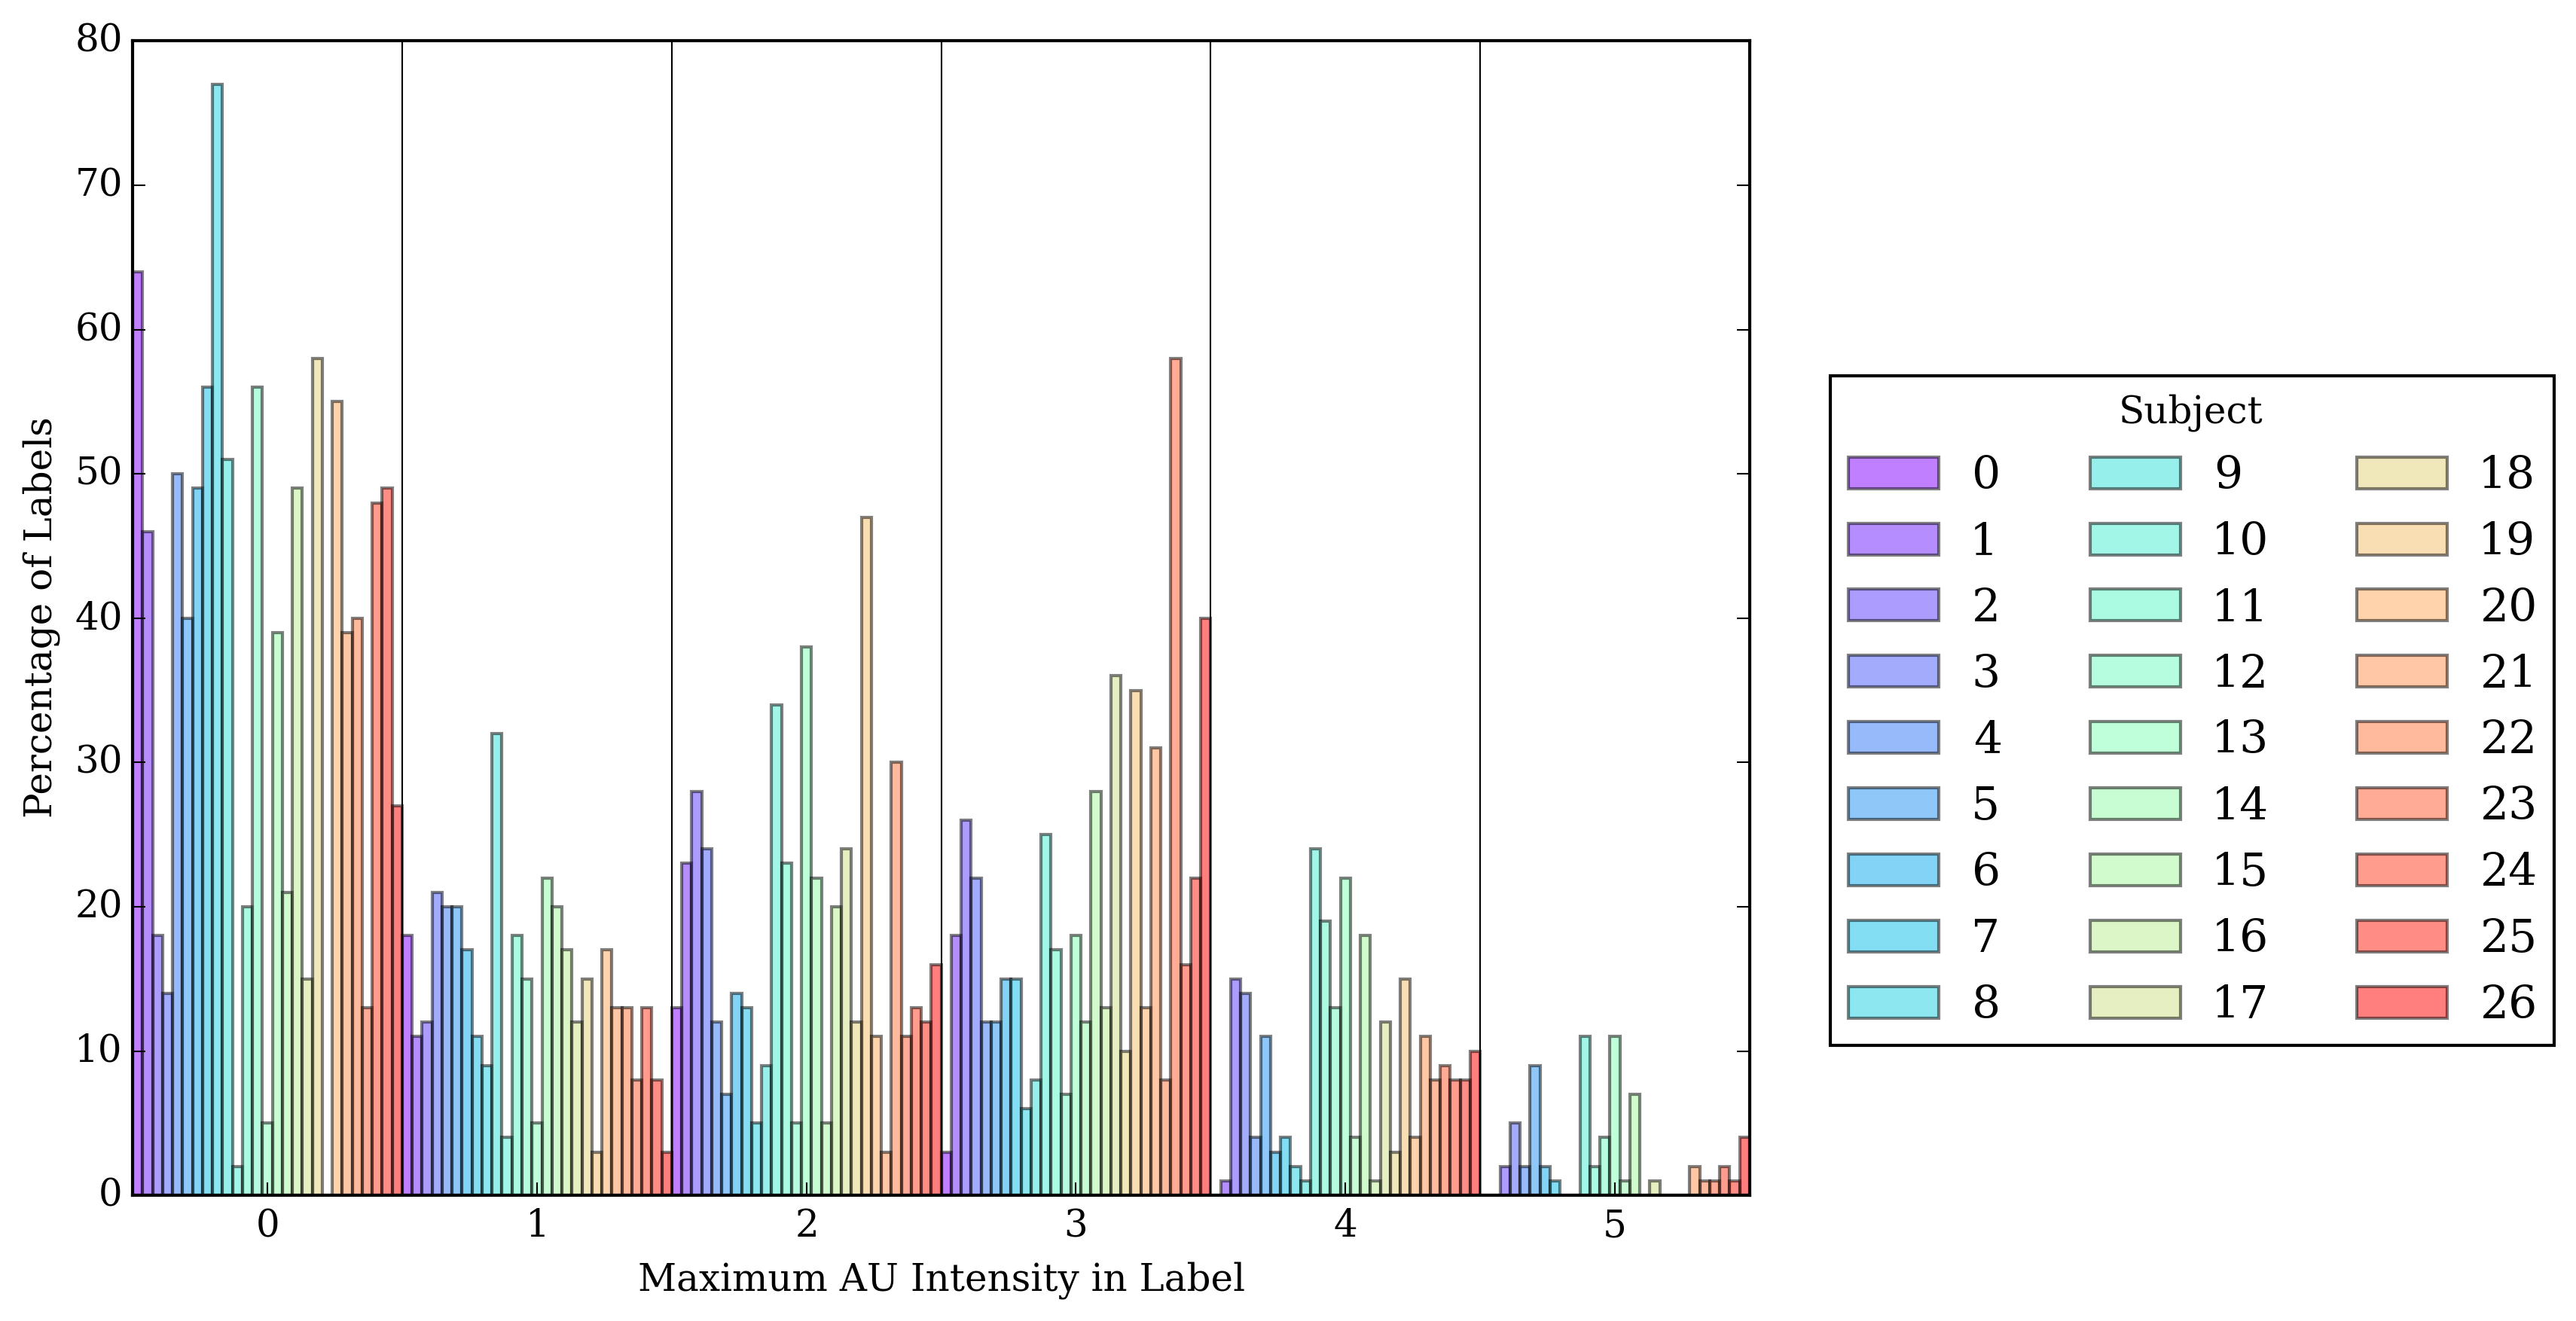
\includegraphics[width=\textwidth]{../graphs/maximum_label_intensity_disfa.pdf}
  \caption{DISFA dataset: This graph shows what the maximum value in each label is in the DISFA dataset per subject. This
  is done to illustrate the number of labels which contain absolutely no information.}\label{disfastats}
\end{figure}
\newpage

\subsubsection{Deep learning approaches to FAU detection}
It has been shown that deep neural networks containing convolutional, max pooling,
dropout and fully connected layers can effectively learn how to classify AUs in
a selection of datasets \cite{Gudi2015,Ghosh2015,dodeeplearn}. These
works only include networks which ignore the temporal structure of the data,
other architectures do incorporate this \cite{emonet,Jaiswal2016}.


%
%
%






\subsubsection*{Comparison of networks in Table \ref{compnet}}
Network \cite{Ghosh2015} (Ghosh et al.) was trained on CK+, DISFA and BP4D datasets.
A key result of this paper was that they achieved good generalisation between datasets
with classifications accuracies between 60\% and 80\% for these generalisation experiments.
A feature particular to this network was that after the softmax layer, which assigns probabilities
to each AU it uses QDA (Quadratic Discriminant Analysis) \cite{precogbook} to
make predictions about whether AUs are present. A point of interest is also that
mean face normalisation is done per subject and then all for all subjects.

Network \cite{Gudi2015} (Amogh Gudi et al.) was trained on BP4D and SEMAINE
datasets achieving an average F1 score of 0.52 and 0.34 respectively. This paper
uses minimal preprocessing hence is a good example of how CNNs can learn features
with little feature engineering.

Network \cite{dodeeplearn} (Pooya Khorrami et al.) was trained on TFD and CK+,
this got average accuracies of 89.9\% and 98.3\% respectively in detecting emotions. This
is therefore not directly comparable, but they do explore connecting it with AUs.
An interesting point about this work is that they could stimulate activations in the convolutional
layers and directly see that the network had learned different facial actions demonstrating the
power of these networks.

Network \cite{Jaiswal2016} (Shashank Jaiswal et al.) was trained on SEMAINE and
BP4D achieving an overall weighted F1 score of 0.54. Which is on average higher
than network \cite{Gudi2015} as claimed in the paper. This paper includes a lot more
prior knowledge than the others, firstly it uses a BLSTM to incorporate temporal structure
and it defines multiple input streams from each facial region, allowing the convolutional
filters to become more specialised. This is the only paper where they say they use
two outputs for each AU so that the softmax creates a probability distribution for
each AU and not for all of them at once.

It should be noted that it is difficult to compare the performance between these
networks as they all use different evaluation scores as shown in table \ref{compscore}.

\begin{table}[h!]
\centering
{\footnotesize
\begin{tabular}{|lllllllll|}
\hline
Network                      & \multicolumn{2}{c}{Ghosh et. al\cite{Ghosh2015}}                         & \multicolumn{2}{c}{Gudi et. al.\cite{Gudi2015}}                            & \multicolumn{2}{c}{Khorrami et. al.\cite{dodeeplearn}}                          & \multicolumn{2}{c|}{Jaiswal et. al.\cite{Jaiswal2016}}   \\ \hline
\multicolumn{1}{|l|}{Element} & Type     & \multicolumn{1}{l|}{Dimensions}                    & Type     & \multicolumn{1}{l|}{Dimensions}                      & Type          & \multicolumn{1}{l|}{Dimensions}                  & Type      & Dimensions                     \\ \hline
\multicolumn{1}{|l|}{x}       &          & \multicolumn{1}{l|}{$40\times40\times1$}           &          & \multicolumn{1}{l|}{$48\times 48\times1$}            &               & \multicolumn{1}{l|}{$96\times96\times1$}         &           & $?\times?\times1$              \\ \hline
\multicolumn{1}{|l|}{$L_1$}   & conv 1   & \multicolumn{1}{l|}{$12\times 12\times1\times 70$} & conv 1   & \multicolumn{1}{l|}{$5\times 5\times1\times64$}      & conv 1        & \multicolumn{1}{l|}{$5\times5\times1\times64$}   & conv 1*   & $5\times5\times(2n+1)\times32$ \\
\multicolumn{1}{|l|}{$y_1$}   &          & \multicolumn{1}{l|}{$29\times29\times70$}          &          & \multicolumn{1}{l|}{$44\times44\times64$}            &               & \multicolumn{1}{l|}{$92\times92\times64$}        &           & $?\times?\times32$             \\ \hline
\multicolumn{1}{|l|}{$L_2$}   & max pool & \multicolumn{1}{l|}{$2\times 2$}                   & max pool & \multicolumn{1}{l|}{$3\times3$ (stride 2)}           & max pool      & \multicolumn{1}{l|}{$2\times2$}                  & max pool*  & $3\times3$                    \\
\multicolumn{1}{|l|}{$y_2$}   &          & \multicolumn{1}{l|}{$15\times15\times 70$}         &          & \multicolumn{1}{l|}{$22\times 22\times64$}           &               & \multicolumn{1}{l|}{$46\times46\times64$}        &           & $?\times?\times32$             \\ \hline
\multicolumn{1}{|l|}{$L_3$}   & conv 2   & \multicolumn{1}{l|}{$4\times 4\times70\times 10$}  & conv 2   & \multicolumn{1}{l|}{$5 \times 5 \times 64\times64$}  & conv 2        & \multicolumn{1}{l|}{$5\times5\times64\times128$} & conv 2    & $5\times5\times32\times64$     \\
\multicolumn{1}{|l|}{$y_3$}   &          & \multicolumn{1}{l|}{$12\times 12 \times 10$}       &          & \multicolumn{1}{l|}{$18 \times 18\times64$}          &               & \multicolumn{1}{l|}{$42\times42\times128$}       &           & $?\times?\times64$             \\ \hline
\multicolumn{1}{|l|}{$L_4$}   & max pool & \multicolumn{1}{l|}{$2\times 2$}                   & conv 3   & \multicolumn{1}{l|}{$4\times 4 \times64 \times 128$} & max pool      & \multicolumn{1}{l|}{$2\times2$}                  & conv 3    & $5\times5\times64\times64$     \\
\multicolumn{1}{|l|}{$y_4$}   &          & \multicolumn{1}{l|}{$6\times 6 \times 12$}         &          & \multicolumn{1}{l|}{$15\times15\times128$}           &               & \multicolumn{1}{l|}{$21\times21\times128$}       &           & $?\times?\times64$             \\ \hline
\multicolumn{1}{|l|}{$L_5$}   & fc       & \multicolumn{1}{l|}{$500$}                         & fc       & \multicolumn{1}{l|}{$3072$}                          & conv 3        & \multicolumn{1}{l|}{$5\times5\times1\times256$}  & conv 3    & $4\times4\times64\times128$    \\
\multicolumn{1}{|l|}{$y_5$}   &          & \multicolumn{1}{l|}{$500$}                         &          & \multicolumn{1}{l|}{$3072$}                          &               & \multicolumn{1}{l|}{$17\times17\times256$}       &           & $?\times?\times128$            \\ \hline
\multicolumn{1}{|l|}{$L_6$}   & fc       & \multicolumn{1}{l|}{$100$}                         & softmax  & \multicolumn{1}{l|}{$12$}                            & quadrant pool & \multicolumn{1}{l|}{}                            & fc        & $3072$                         \\
\multicolumn{1}{|l|}{$y_6$}   &          & \multicolumn{1}{l|}{$100$}                         &          & \multicolumn{1}{l|}{$12$}                            &               & \multicolumn{1}{l|}{$4\times4\times256$}         &           & $3072$                         \\ \hline
\multicolumn{1}{|l|}{$L_7$}   & softmax  & \multicolumn{1}{l|}{$12$}                          &          & \multicolumn{1}{l|}{}                                & fc            & \multicolumn{1}{l|}{$300$}                       & softmax   & $2N_{C}$                       \\
\multicolumn{1}{|l|}{$y_7$}   &          & \multicolumn{1}{l|}{$12$}                          &          & \multicolumn{1}{l|}{}                                &               & \multicolumn{1}{l|}{$300$}                       &           & $2N_{C}$                       \\ \hline
\multicolumn{1}{|l|}{$L_8$}   & QDA      & \multicolumn{1}{l|}{}                              &          & \multicolumn{1}{l|}{}                                & softmax       & \multicolumn{1}{l|}{$8$}                         & BLSTM     &                                \\
\multicolumn{1}{|l|}{$y_8$}   &          & \multicolumn{1}{l|}{}                              &          & \multicolumn{1}{l|}{}                                &               & \multicolumn{1}{l|}{$8$}                         &           &                                \\ \hline
\end{tabular}

\caption{A comparison of network architectures from the literature, all networks
use RELUs as their activation functions apart from in the final layer where it is
typical to use a softmax. $x$ denotes the input image, $L_i$ denotes the $i$th layer and $y_i$ denotes the output of the $i$th layer.
$N_{C}$ is the number of classes.
The question marks signify the dimensions of input images are variable as it depends on the input stream. fc is for fully connected and
conv is for convolutional layer. QDA is Quadratic Discriminant Analysis and BLSTM is for Bidirectional Long Short-Term Memory neural
networks.
\newline
*These layers are per input stream} \label{compnet}

}
\end{table}

\begin{table}[h!]
\centering

\begin{tabular}{lcccc}
\hline
Score    & \multicolumn{1}{l}{Ghosh et. al\cite{Ghosh2015}} & \multicolumn{1}{l}{Network Gudi2015} & \multicolumn{1}{l}{Gudi et. al.\cite{Gudi2015}} & \multicolumn{1}{l}{Khorrami et. al.\cite{dodeeplearn}} \\ \hline
Accuracy & \checkmark                            &                                      &                                         & \checkmark                              \\
F1       &                                       & \checkmark                           & \checkmark                              &                                         \\
AUC      &                                       &                                      &                                         &                                         \\
2AFC     & \checkmark                            &                                      & \checkmark                              &                                         \\ \hline
\end{tabular}
\caption{A comparison of which evaluation methods were used in a selection of papers.} \label{compscore}
\end{table}

\begin{table}[h!]
\centering

\begin{tabular}{lcccc}
\hline
Dataset  & \multicolumn{1}{l}{Ghosh et. al\cite{Ghosh2015}} & \multicolumn{1}{l}{Network Gudi2015} & \multicolumn{1}{l}{Gudi et. al.\cite{Gudi2015}} & \multicolumn{1}{l}{Khorrami et. al.\cite{dodeeplearn}} \\ \hline
CK+      & \checkmark                            &                                      &                                         & \checkmark                              \\
DISFA    & \checkmark                            &                                      &                                         &                                         \\
SEMAINE* &                                       & \checkmark                           & \checkmark                              &                                         \\
BP4D*    & \checkmark                            & \checkmark                           & \checkmark                              &                                         \\
TFD      &                                       &                                      &                                         & \checkmark                              \\ \hline
\end{tabular}
\caption{A comparison of which datasets were used in a selection of papers.} \label{compdat}
\end{table}

\subsubsection{Deep Learning Framework}
Tensorflow \cite{tensorflow} was chosen as the deep learning framework for this
project. Many others exist, some advantages that tensorflow has over its rivals
includes platform independence, distributed computing and inbuilt visualisation
of network topology and parameters over time. As most other frameworks it uses python
to define it's computations and also includes a C++ interface.




%
%
%
\subsection{Theory}
\subsubsection{Artificial Neural Networks}
An artificial neuron is a function which takes in a vector of inputs, computes their
weighted sum and applies a non-linearity as follows:
\begin{equation}
    a(\mathbf{x}) = \sigma \left ( \sum_{i=1}^N w_ix_i + b \right )
\end{equation}
Here $\sigma$ is a scalar function, $w_i$ is a scalar weight and $b$ is its bias. $N$ is the size of the input and weight vector.
These neurons can be combined into layered networks to construct artificial neural networks.
The weights $w$ can then be rewritten as matrices $\mathbf{W}$ which define how
activations from one layer are transferred to the next\footnote{Note: when a vector
is put into a scalar function it is assumed that it acts on each element of
the vector. The only exception is with the softmax.}.
\begin{equation}
    \mathbf{a}(\mathbf{x}) = \mathbf{\sigma} \left ( \mathbf{W}\mathbf{x} + \mathbf{b} \right )
\end{equation}

Popular activation functions include:
\begin{multicols}{2}


\begin{equation}
\text{The sigmoid:}\quad
  \sigma (x) = \frac{1}{1-e^{-x}}
\end{equation}


\begin{equation}
\text{The ReLU:}\quad
\sigma(x) =
\begin{cases}
      x & x\geq 0 \\
      0 & x < 0
   \end{cases}
\end{equation}


\begin{equation}
\text{Hyperbolic tan:}\quad
    \sigma(x)=\frac{e^x - e^{-x}}{e^x + e^{-x}}
\end{equation}


\begin{equation}
\text{The softmax:}\quad
  \sigma(\mathbf{x})_j = \frac{e^{x_j}}{\sum_i e^{x_i}}
\end{equation}


\end{multicols}

\begin{figure} \label{disfagraph}
    \center
  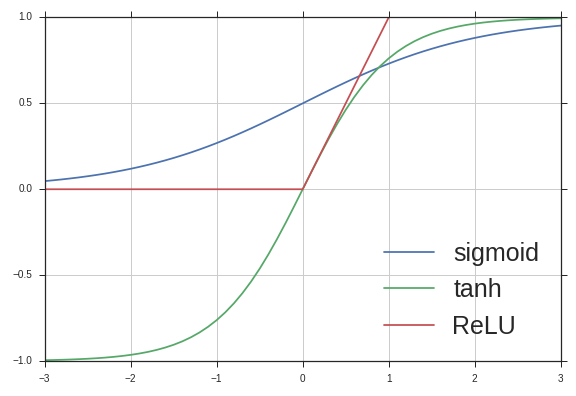
\includegraphics[width=.5\textwidth]{../graphs/actfuncs.pdf}
  \caption{Comparison of common activation functions for neural networks}
\end{figure}



An $N$ layer network can
then be thought of as a function with a recursive structure (these are also known as fully connected layers):
\begin{equation}
    \mathbf{y} = \mathbf{a}_{N}(\mathbf{a}_{l-1}(...\mathbf{a}_1(\mathbf{x})...))
\end{equation}
Now assuming there exists a set of $\tilde{\mathbf{x}}$ and $\tilde{\mathbf{y}}$ which make
up a training data set, these could be sets of images and labels, then a cost function
to optimise can be defined:
\begin{equation}
    J(\tilde{\mathbf{x}},\tilde{\mathbf{y}}) = \frac{1}{N}\left |\mathbf{y}(\tilde{\mathbf{x}})-\tilde{\mathbf{y}}\right | ^2
\end{equation}
this is called the least mean squared error, another popular cost function is
the cross entropy:
\begin{equation}
    J(\tilde{\mathbf{x}},\tilde{\mathbf{y}}) = -\frac{1}{N}\tilde{\mathbf{y}}\cdot\log(\mathbf{y}(\tilde{\mathbf{x}}))
\end{equation}

The derivative of these cost functions can then be computed in order to minimise it.
The simplest way is to do this is per training example, however stochastic gradient
descent\cite{Amari1993} has emerged as a superior method. Simply put it computes the gradient with respect
to many randomly drawn samples, it has the advantage of following a smoother path
towards the local minimum.
\subsubsection*{Convolutional Layers}
A convolutional layer is a generalisation of simple fully connected layers described
above. It consists of a set of $K$ filters of size $m\times m$, which are applied to the input to produce
a set of $K$ outputs. The filters are applied with a 2D convolution.


To describe them, firstly assume that any vector described in the previous section
can also be rewritten as a matrix, i.e $\mathbf{x} \in \mathbb{R}^{n}
\rightarrow \mathbf{x} \in \mathbb{R}^{N \times M} \quad NM=n$, in practice this is made
easy by using numbers which factorise well.

Then the following equation describes the output of a convolutional layer:
\begin{equation} \label{CNN}
    \mathbf{a}(\mathbf{x})_{ijk} = \sigma \left ( \sum_{a=0}^{m-1}\sum_{b=0}^{m-1}(w_{abk}x_{(i+a)(j+b)k}) + b_k \right )
\end{equation}
Here $i,j$  denote row, column indices for the matrix (image) $\mathbf{x}$, $k$ is the filter index, $w_{abk}$
gives the filter element and $b_k$ is the bias for that filter. This is done for all $K$ filters.

One issue is how to deal with indices which are out of bounds, SAME padding can be used which sets out of bounds
elements to zero and so preserves the image size or VALID can be used, this keeps the filter within the bounds of the
image and hence the output is of a smaller dimension. Lastly a stride greater than 1 can be incorporated into equation
\ref{CNN} meaning that $\mathbf{a}$ is only computed for a fraction of indices $i,j$.
% \begin{equation}
% 	C : \mathbb{R}^{n\times m \times p \times l} \rightarrow \mathbb{R}^{N\times M \times l \times K}
% \end{equation}
%con%
\subsubsection*{Max Pooling Layers}
A max pooling layer simply splits its input into a set of sections and extracts
the highest value from each. It is a simple but effective method to down sample
an image, it helps to keep the computational overhead of these algorithms
down. However a recent trend \cite{Springenberg2015} has emerged where max pooling
layers are not used, instead a convolutional layer with a large stride accomplishes
the same amount of down-sampling.
\subsubsection*{Dropout Layers}
A layer with dropout applied to it randomly turns neurons off, making it more
difficult for the network to overfit data. There is a dropout probability
which determines how often neurons are disabled, it is typically under 20\%
\subsubsection{Autoencoders}
An autoencoder is at its bare minimum a artificial neural network which tries
to reproduce its input as accurately as possible. So the cost function for the
least mean squared error becomes:

\begin{equation}
    J(\tilde{\mathbf{x}},\tilde{\mathbf{y}}) = \frac{1}{N}\left |\mathbf{y}(\tilde{\mathbf{x}})-\tilde{\mathbf{x}}\right | ^2
\end{equation}

Constraints are
placed on the network so that it has to learn to compress the input, the following
are popular constraints that may be used:
\begin{itemize}
    \item Few neurons in the hidden layers
    \item Sparsity: the average activation of the neurons can be kept under a
    threshold, typically a small value close to zero \cite{autong}
    \item Noise may be added to the input, this makes the network more likely
    to learn general features.
\end{itemize}
Lastly there are Variational Autoencoders which combine ideas from Bayesian inference
to create networks which can not only reconstruct their input but also act as a
distribution which can be sampled from, allowing for the generation of new samples \cite{Kingma2013}.

\subsubsection{Stacked Autoencoder}

A stacked autoencoder is typically used for pre-training a network for a classification task.
Instead of training the whole structure at once, each layer is trained as the last hidden
layer of some temporary autoencoder. It has been shown that this can improve classification performance \cite{stacks}.


\subsubsection{Convolutional Autoencoder}
A convolutional autoencoder works in the same way as a standard autoencoder, however
undoing the max pooling presents a problem, as a max pooling layer throws away
information, its inverse will never be exact. The following strategies have been
used with success:
\begin{itemize}
    \item Replacing each entry with an $n \times n$ matrix filled with the original
    entry.
    \item Replacing each entry with an  $n\times n$  matrix with
    the original entry in the upper left and the other squares set to 0. \cite{Dosovitskiy2015}
\end{itemize}

Other than that all other elements have very straightforward inverses and hence
a convolutional autoencoder can be constructed.

\subsubsection{Model Evaluation}
With any kind of classification model it is crucial to be able to evaluate its
performance, in a standard and reproducible way. For the problem of classifying
AUs the simplest case is to split the problem into a set of $n_C$ decision problems
where $n_C$ is the number of distinct classes. Now the problem is reduced to
evaluating the performance of a binary classifier. Finding the confusion matrix is
the first step in such a problem. For a binary problem it is defined as follows:
\begin{equation}
C =
\begin{pmatrix}
TP & FN\\
FP & TN
\end{pmatrix}
\end{equation}
Where $TP$ is the number of true positives, $FN$ is the number of false negatives
, $FP$ is the number of true positives and $TN$ is the number of true negatives.
In a perfect classification, this matrix would have $FP=FN=0$, however this is rare
and we can define quantities to measure how close to this ideal we are. Note we
only define the binary case here, the more general confusion matrix for multiple
classes can easily be defined but is not relevant here.
\begin{equation}
\text{Recall} = \frac{TP}{TP+FN}
\end{equation}
\begin{equation}
\text{Precision} = \frac{TP}{TP+FP}
\end{equation}
\begin{equation}
\text{F1} = 2 \cdot \frac{\text{Recall} \cdot \text{Precision}}{\text{Recall} + \text{Precision}}
\end{equation}

Hence recall is decreased by false negatives, i.e not being able to recall the class
when presented with it. Precision is decreased by false positives i.e stating the class
is present when it is not. Both measures describe a different aspect of the accruacy and so the F1 is the
harmonic mean between these two, it is the quantity this report will seek to maximise and use to compare
results with the literature.

Another useful measure is the area under the Receiver operating characteristic (ROC) curve.
As neural networks output a number between 0 and 1, a threshold must be chosen to signify
when the network declares a class present. By varying this threshold a series of true positive and false positive rate points
can be generated, this is the ROC curve. The area under this is ideally 1 and in the worst case 0, hence this is
another measure of classification accuracy that is invariant to the chosen threshold.

%
%
%
\newpage
\section{Progress Report}
%
%
%
A prototype with all key functionality has been completed, apart from
the autoencoder section of the network. However this has been tested
in a separate program and hence adding it should not pose a difficulty.

Most effort has been concentrated on getting the model evaluation
to be reliable and useful so that it is easy to see what is going on
inside the model.

The following datasets have been used with the prototype:
\begin{itemize}
 \item The MNIST Database of handwritten digits \cite{mnist} : although
       unrelated to the problem of facial recognition, this is used to initially
       validate that prototype networks are functional. It contains 70,000 images of
       digits between 0-9.
    \item The DISFA database \cite{disfa}, see section \ref{disfa_list}
\end{itemize}

The following information is generated for each run:
\begin{itemize}
    \item Per training epoch for train and validation set but per threshold for the test set:
            \begin{itemize}
                \item Precision
                \item Recall
                \item F1 Score
                \item Area under ROC
            \end{itemize}
  \item Cost functions, least mean squared and cross-entropy per training epoch
  \item Weights, biases and activations of the network per training epoch
\end{itemize}

\subsection{Example graphs generated when training a network on MNIST}

This network had one convolutional layer of size $5\times5\times1\times64$ and one
fully connected layer of size $100$ connected to the output of size $10$. It was
trained using the cross-entropy cost function and using an Adam optimizer\cite{adam} with learning rate $0.001$.



\begin{multicols}{2}
\begin{Figure}
 \centering
 \includegraphics[width=.9\textwidth]{graphs/cross_entropy.pdf}
 \captionof{figure}{The cross-entropy as a function of training epoch for the training and validation set}
\end{Figure}

\begin{Figure}
 \centering
 \includegraphics[width=.9\textwidth]{graphs/lmsq.pdf}
 \captionof{figure}{The least mean squared error as a function of training epoch for the training and validation set.
 Note that even though this was not the objective function it still decreases and converges at a similar time to the cross entropy}
\end{Figure}

\begin{Figure}
 \centering
 \includegraphics[width=.9\textwidth]{graphs/test_per_au.pdf}
 \captionof{figure}{Accuracy information for the test set.The horizontal axes here are training epochs. The colours correspond to digits in the MNIST dataset.}
\label{test}
\end{Figure}

\begin{Figure}
 \centering
 \includegraphics[width=.9\textwidth]{graphs/train_per_au.pdf}
 \captionof{figure}{Accuracy information for the training set. The horizontal axes here are training epochs. The colours correspond to digits in the MNIST dataset.}
\end{Figure}

\begin{Figure}
 \centering
 \includegraphics[width=.9\textwidth]{graphs/validation_per_au.pdf}
 \captionof{figure}{Accuracy information for the validation set. The horizontal axes are the threshold instead of the training epoch here. The colours correspond to digits in the MNIST dataset.}
\end{Figure}

\end{multicols}


It is evident the network generally performs well, apart from when recognising the digit 1. This is mainly due to the fixed threshold value of 0.5, looking at figure \ref{test}
it is possible to see that 0.2 is roughly the optimum threshold for the 1 digit. These are the kinds of experiments that need to be performed on the DISFA dataset and
an autoencoder will be added. There has been some preliminary work with the DISFA set but some bug fixes are still to be completed.

\subsection{Conclusion}

An autoencoder classifier  network has been tried on the MNIST dataset and no obvious improvement
was seen, however this is not the best test as the MNIST dataset is already very easy to model.

Currently the autoencoder has not been tried with larger convolutional networks or with DISFA,
this is because it is still a priority to reproduce the classification rates in the literature
with a standard deep network.

With the bulk of the coding out of the way results should start coming in at a faster rate.

%
%
%
\section{Plan}
\subsection{Minimum Objectives}
\begin{enumerate}
  \item Match performance benchmarks in the literature without the autoencoder
  \item Improve model evaluation on existing prototype.
  \item Investigate whether the autoencoder can improve classification accuracy
\end{enumerate}
\subsection{Full Objectives}
\begin{enumerate}
  \item Theorise whether stacked, sparse and de-noising autoencoders may
        be useful for the problem.
  \item Test how well the trained networks generalize to other datasets
  \item Clarify how the proposed method differs from standard pre-training of
        neural networks and discuss whether it is a novel approach.
  \item Improve on classification rates seen in the literature for the DISFA and CK+ datasets
\end{enumerate}
\subsection{Extensions}
\begin{enumerate}
  \item Use some Bayesian Optimisation to learn hyperparameters which increase
        the initial gradient of the cost function (pybo)
  \item Implement and research other unsupervised methods such as variational
        autoencoders and RMBs
  \item Visualise the features learnt by the convolutional network and compare
        to the literature
\end{enumerate}


\bibliographystyle{unsrt}
\bibliography{bib/autofaces}
\end{document}
